\documentclass[conference]{IEEEtran}
\IEEEoverridecommandlockouts
% The preceding line is only needed to identify funding in the first footnote. If that is unneeded, please comment it out.
\usepackage{cite}
\usepackage{amsmath,amssymb,amsfonts}
\usepackage{algorithm}
\usepackage{algpseudocode}
\usepackage{graphicx}
\usepackage{textcomp}
\usepackage{xcolor}
\usepackage{listings}
\usepackage{url}
\begin{document}


\title{Dynamic Load Balancing of Plasma and Flow Simulations\\
\thanks{
This research was supported by the National Science Foundation under Grant No.
ACI 1533581, (SI2-SSE: Fast Dynamic Load Balancing Tools for Extreme Scale
Systems) and the U.S. Department of Energy, Office of Science, under awards
DE-AC52-07NA27344 (FASTMath SciDAC Institute) and DE-SC0018275 (Unstructured
Mesh Technologies for Fusion Simulation Codes). Any opinions, findings, and
conclusions or recommendations expressed in this material are those of the
author(s) and do not necessarily reflect the views of the National Science
Foundation.
}}

\author{\IEEEauthorblockN{1\textsuperscript{st} Gerrett Diamond}
\IEEEauthorblockA{\textit{SCOREC} \\
\textit{Rensselaer Polytechnic Institute}\\
\textit{Institute}\\
Troy, NY\\
diamog@rpi.edu}
\and
\IEEEauthorblockN{2\textsuperscript{nd} Cameron W. Smith}
\IEEEauthorblockA{\textit{SCOREC} \\
\textit{Rensselaer Polytechnic}\\
\textit{Institute}\\
Troy, NY\\
smithc11@rpi.edu}
\and
\IEEEauthorblockN{3\textsuperscript{rd} Eisung Yoon}
\IEEEauthorblockA{
\textit{Ulsan National Institute}\\
\textit{of Science and Technology}\\
Ulsan, South Korea\\
esyoon@unist.ac.kr}
\and
\IEEEauthorblockN{4\textsuperscript{rd} Mark S. Shephard}
\IEEEauthorblockA{\textit{SCOREC} \\
\textit{Rensselaer Polytechnic}\\
\textit{Institute}\\
Troy, NY\\
shephard@rpi.edu}
}

\maketitle

\begin{abstract}
  Extracting performance from simulations with complex information dependencies
  on massively parallel computers requires the computational work to be evenly
  distributed across the processing resources while maintaining low
  communication costs.
  Plasma simulations using a particle-in-cell method and computational fluid
  dynamics using unstructured mesh-based finite element and volume
  methods present three distinct distribution requirements.
  To meet these needs, we present EnGPar's diffusive partition improvement
  method.
  An initial demonstration of EnGPar's particle distribution improvement is
  provided along with fluid dynamics mesh partition improvement results on up to
  512Ki processes on an IBM BlueGene/Q.
\end{abstract}

\begin{IEEEkeywords}
partition improvement, multigraph, hypergraph, dynamic load balancing,
particle-in-cell, computational fluid dynamics, plasma physics
\end{IEEEkeywords}

\section{Introduction}

High performance computing applications have a wide range of partitioning
requirements for managing computation and communication costs. For evolving simulations these
costs change as the simulation proceeds. In order to maintain good performance throughout the
simulation, quick repartitioning methods are required that can deal with incremental changes
to the computational load.

In plasma physics simulations using a particle-in-cell (PIC) method and finite
element/volume based computational fluid dynamics (CFD), unstructured meshes are utilized
as a discretization of the spatial domain of interest. The partitioning of the
mesh into sets of elements assigned to a process, a part, results in
computational costs associated with the mesh entities and communication
costs relative to the number of shared entities between parts. In addition to
these basic metrics, applications add further criteria that are critical for performance.

Multilevel graph/hypergraph methods and geometric methods have been successfully
applied to balance unstructured mesh applications.
Multilevel graph/hypergraph methods are the most powerful tools to build good static
partitions~\cite{catalyurek2013umpa,karypis1999parallel,lasalle2013multi,schloegel2002parallel}.
These methods construct a graph representing the data of the application. Then, target
reducing the imbalance (measured as max divided by average) of the graph vertices while
minimizing the edges cut between processes. Multilevel methods are very good at reducing
these metrics, but require increasing amounts of memory as they are applied to
larger part counts. One way to alleviate these costs is to run multilevel partitioners globally
out to thousands of processes, then partition locally on each of those parts to go out
further. This approach readily supports partitions with millions of parts, but each
local partitioning cannot improve the global partitioning. For meshes, these methods
can degrade the final load balance which is a function of not only base mesh
entity count, but of a number of mesh level
interactions~\cite{zhou2012unstructured,SmithParma2015}.

Geometric methods quickly provide a spatial partition. They are good for getting low
imbalances of a single criteria, but often result in poor surface areas of parts and thus large
communication costs in the
applications~\cite{devineMultiJagged2015,bergerRib1987}.

In order to improve the partitions for PIC and CFD applications, we utilize diffusive
load balancing procedures to improve the partitions. Diffusive methods iteratively transfer
weight from heavily loaded parts to lighter neighboring parts
\cite{cybenko1989dynamic,subramanian1994analysis}. Diffusive methods have been shown to be
able to reduce the large imbalances accounting for a full set of mesh entity
considerations~\cite{SmithParma2015}. Our tool, EnGPar, uses diffusive methods on a
generalized graph structure in order to improve partitions for a diverse set of application needs.

Section~\ref{sec:engpar} briefly discusses EnGPar.
Section~\ref{sec:pic} discusses a PIC application and initial results
using EnGPar. Section~\ref{sec:cfd} describes two different types of CFD codes. Results for CFD
mesh partitions are given in Section~\ref{sec:results}.
A brief summary of the results closes the paper.

\section{EnGPar} \label{sec:engpar}

%\begin{itemize}
%\item Discuss the Ngraph in general graph terms with some figures
%\item Discuss the construction for a element-partitioned mesh as an example with figure
%\item Discuss dynamic load balancing and the general diffusive steps
%\end{itemize}

EnGPar~\cite{engparSC17,engpar_github} is a tool for partition improvement and
dynamic load balancing.
EnGPar utilizes a multi-hypergraph, called the N-graph, to represent the data of
an application in a relational format that allows load balancing of the vertices
and edges simultaneously.
The N-graph is defined as $G^n = \{V, H^n, P^n\}$ where
$V$ is the set of vertices in the graph. The vertices are uniquely assigned to
processes and are used to represent the main source of data in an application.
$H^n = \{H_1, ..., H_n\}$ are sets of hyperedges where each hyperedge connects a
subset of vertices in $V$. The pins, $P^n = \{P_1,...,P_n\}$, represent the connections from
vertices to hyperedges. Each application that utilizes EnGPar represents the data
that needs partitioning as an N-graph before running any of the partitioning tools.
The general design of the N-graph allows easy representation for different applications
that use structures such as meshes, graphs, and other relational structures.

EnGPar's partition improvement is driven by local diffusive techniques that migrate weight
from heavily weighted parts to lightly weighted parts. This is done by iteratively running
a set of steps until the target imbalance is met or no further improvements are found.
A diffusive iteration consists of three steps: targeting, selection, and migration.
The targeting step consists of gathering information about the current partition and deciding
which neighbors should be sent weight and how much weight to send. The selection step constructs
a plan of what vertices should be sent to each neighbor in order to satisfy the weights in
the targeting step. The final step, migration, is where the vertices are sent to their
destinations and the partition is changed.

\section{Plasma Simulation} \label{sec:pic}

Plasma physics simulated using a PIC method utilize particles
in the spatial domain of a mesh.
In this work we focus on load balancing the computationally dominant particle
push operation that is common to both PIC codes with a fixed field (e.g., GITR~\cite{younkin2017})
and a self-consistent field (e.g., XGC~\cite{chang2004numerical,Ku2016467,ku2009},
M3D-C1~\cite{jardin2012multiple}, HPIC~\cite{hpic2017}).
Given initial electric and magnetic fields on the mesh, the value of the field
for each particle is determined via interpolation from associated mesh vertices.
The spatial position of the particles is then updated using a push operation.
Particle properties are then interpolated back to the mesh vertices; the reverse
of the vertex-to-particle interpolation process.
Unless the entire mesh is replicated on all processes, particles that do not
have their field dependencies satisfied will need to be
sent to a different process that has sufficient field information.
As these simulations continue the particles migrate through the mesh causing
computational imbalance that degrades
performance~\cite{carmona1997,plimptonPic2003,worleyBalancePic2016}.

XGC is a gyrokinetic PIC code for plasma turbulence simulation in a tokamak
fusion device~\cite{chang2004numerical,Ku2016467,ku2009}.
In this work we refer to a development version of XGC named XGCm that supports
a mesh-based particle distribution strategy.
XGCm decomposes the domain with a 2D mesh of the
polodial plane that is repeated a given number of times in the toroidal direction.
Figure~\ref{fig:xgcmPtn}-a depicts a simplified representation of the tokamak computational
domain, the polodial planes that decompose it in the toroidal direction, and the
definition of physics-based geometric features within the planes.
Specifically, Figures~\ref{fig:xgcmPtn}-b and~\ref{fig:xgcmPtn}-c depict the
flux curve and the faces they form. Each flux face is defined as a core and
assigned to a process.
To satisfy information dependencies of particles belonging to the core, the sets
of elements of neighboring cores are replicated and thus avoid communication
during the computationally intensive particle push operation.
These replicated elements are referred to as the buffer region.
Figures~\ref{fig:xgcmPtn}-d and ~\ref{fig:xgcmPtn}-e depict a core and buffer
flux faces that makes up one part. 
This decomposition of the polodial plane is identical for all planes along the
toroidal direction and does does not change during the simulation.

\begin{figure}[!ht]
  \centering
  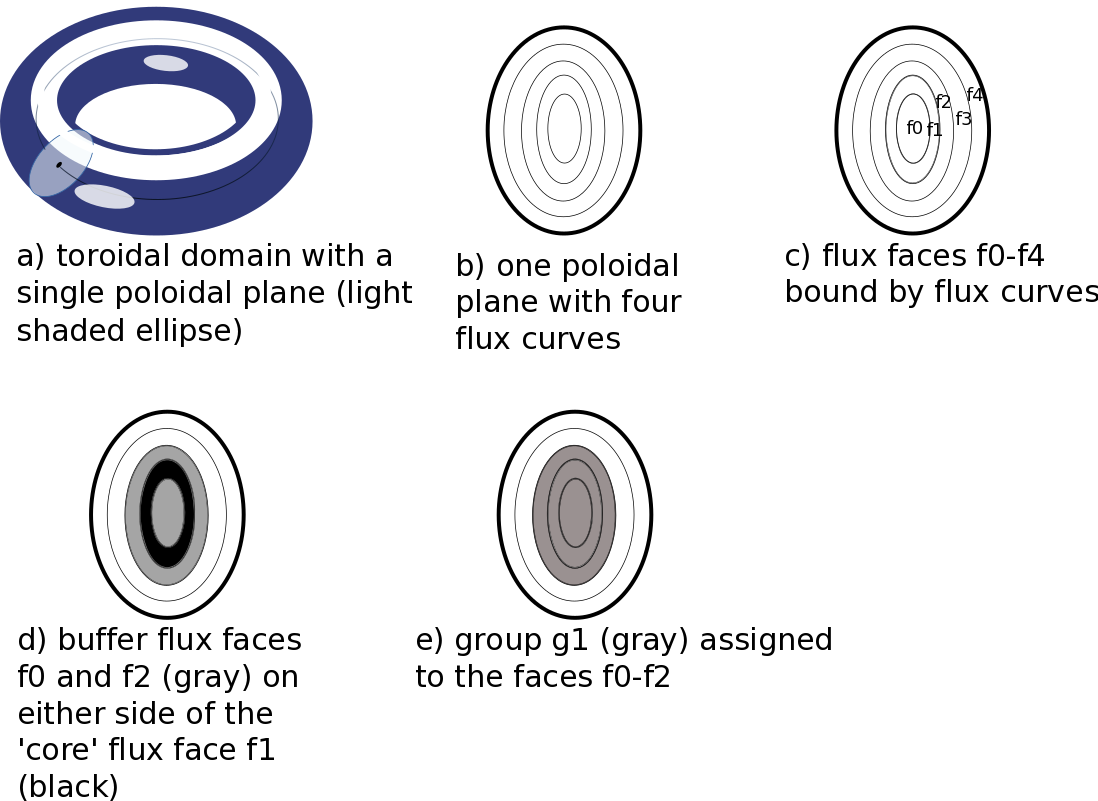
\includegraphics[width=.4\textwidth]{../figures/xgcm_partition.png}
  \caption{XGCm mesh distribution in the toroidal and polodial directions of a tokamak.}
  \label{fig:xgcmPtn}
\end{figure}

The elements in the core flux face of each part, and some layers of the
buffer region elements that surround it, are marked as a safe region.
Within the safe region there is sufficient mesh field information available to
satisfy the dependencies of the push operation.
Initially, particles are distributed uniformly over the tokamak volume.
The dominant motion of the particles, projected to the polodial plane, tends to
keep them within their initial flux face while a secondary motion drifts them
outwards towards the boundary of the plane.
If the particle moves outside of the safe region, it is migrated to a process
where it resides in the safe region before the next push operation.

To ensure that particles are always migrated to the safe elements
of a process, we construct the N-graph carefully such that any partition
decision in EnGPar will always maintain this requirement in XGCm. Towards this,
we represent each region
of overlapping safe zones. Figure \ref{fig:sbars} depicts a model (a) with four flux faces labeled
in (b) as f0-f3. Safe zones for each \texttt{core} are shown in the second row.
Each overlapping safe zone set, $\bar{S_i}$, is in the third row. For an element in
one of the $\bar{S_i}$, the safe zones in the set represent the parts that a particle in
the element can migrate to.

The N-graph is then constructed using the set of $\bar{S_i}$. For each $\bar{S_i}$ a
component is constructed consisting of a hyperedge and vertices for each safe zone
$S_j \in \bar{S_i}$. The hyperedge connects each of the vertices in the component.
The fourth row of Figure \ref{fig:sbars} shows the N-graph components for the example model.
Weights are then applied to each vertex based on the number of particles in the elements
for each part. 
EnGPar is then used in order to determine how to redistribute the weight
associated with particles.

\begin{figure}[!ht]
  \centering
  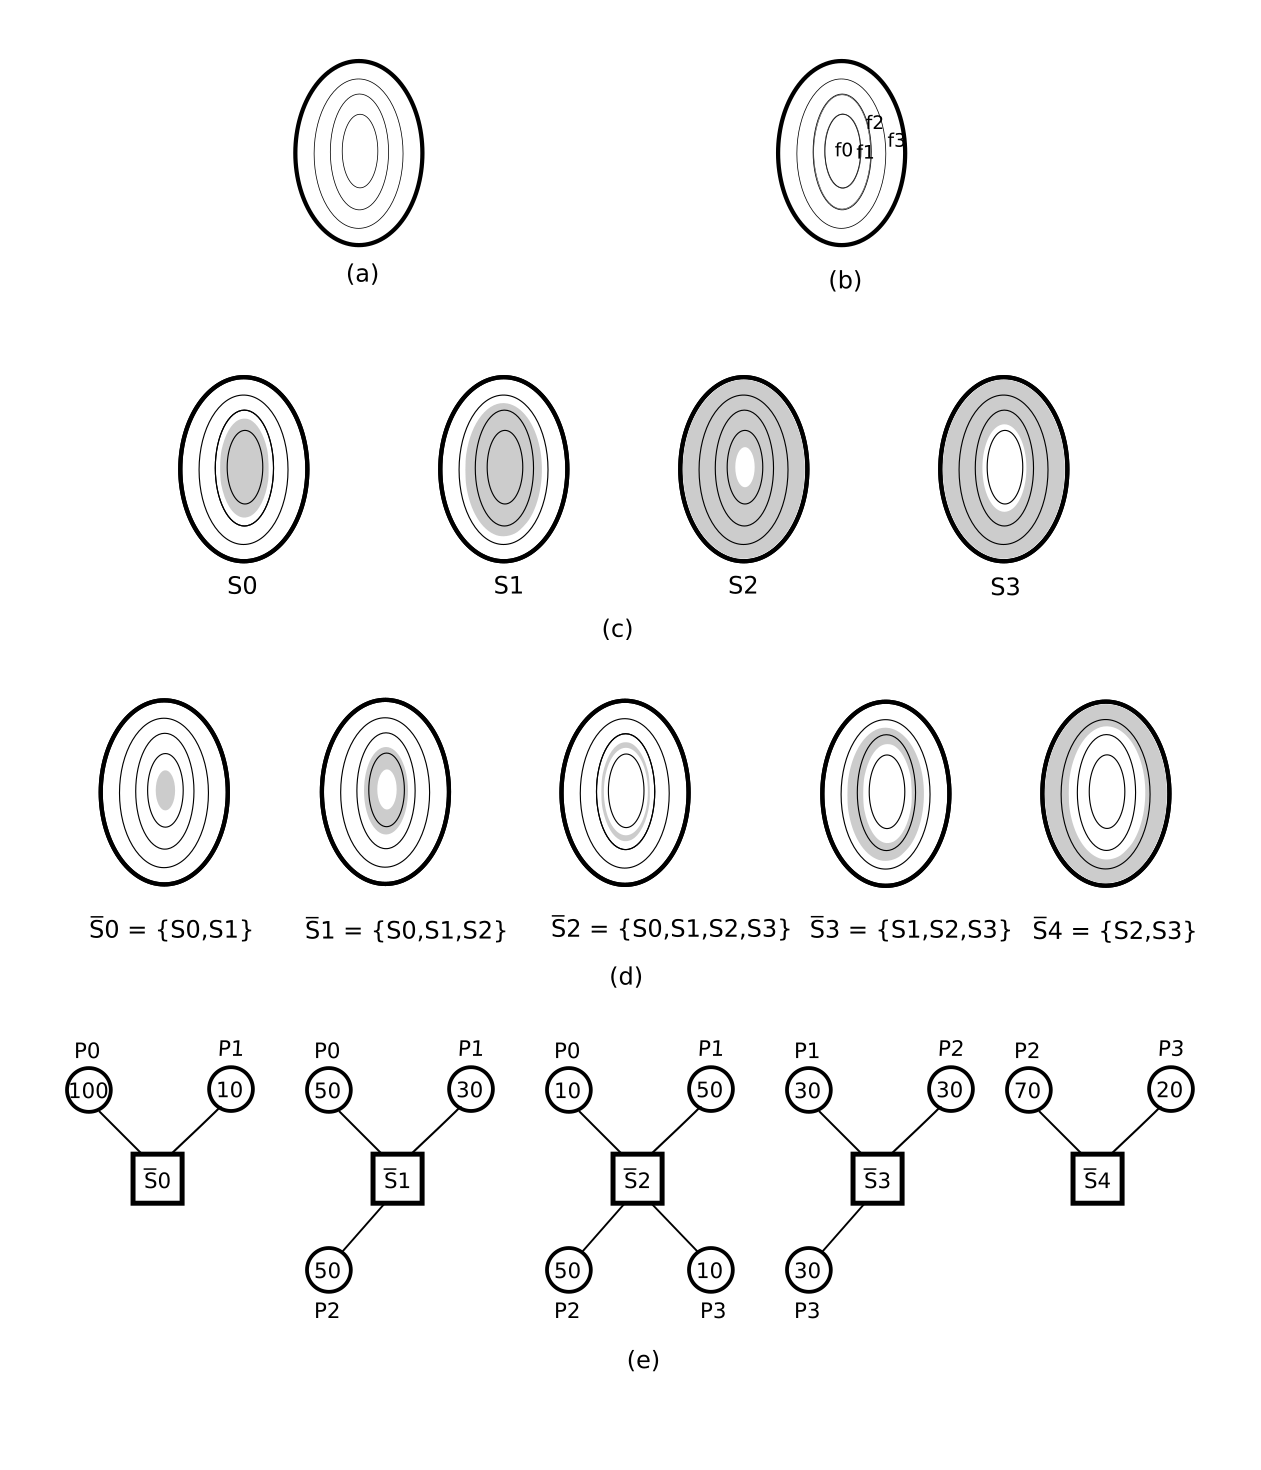
\includegraphics[width=.4\textwidth]{../figures/xgcm_ngraph_construction.png}
  \caption{An example of overlapping safe zones and the N-graph constructed from
  them. A polodial plane (a) with four flux faces, f0-f3 (b). Safe zones around
  each flux face (c). Each overlapping set of safe zones (d) and the N-graph
  constructed from the overlapping safe zones (e). Vertices are represented with
  circles and hyperedges with squares.}
  \label{fig:sbars}
\end{figure}

In order to balance the particles in the mesh, we target redistributing the weights within
each component. We run diffusive techniques on the weights of the vertices
rather than the vertices. This means that instead of migrating graph vertices, we migrate the
weight of the vertices across hyperedges to neighboring vertices to reduce the imbalance
of load in the graph.

After EnGPar's weight diffusion is run, a migration plan is returned that details how
much weight to send from each graph vertex on a part to each of its neighboring vertices.
In XGCm, particles are migrated in order to match the plan. Since each graph vertex was only
connected to processes that could receive the particles from the part, any decision XGCm makes
within the $\bar{S_i}$ will satisfy the requirement of particles being in safe zones. Future work
will go into different particle selection methods that can be applied to reduce how often
dynamic load balancing will be required as particles continue to propagate.

Initial demonstrations of the weighted partitioning approach are run on a 16
process test case. The mesh has around four thousand
mesh faces, four flux faces with four processes per flux face, and sixteen thousand particles.
The initial distribution of particles has an imbalance of 42\%. After running EnGPar, the
imbalance of particles is reduced to 18\%. The push operation's computational load is
statistically proportional to the number of particles on part. thus this
reduction will significantly improve the performance of the computationally
dominant push operation.

\section{Computational Fluid Dynamics} \label{sec:cfd}

Parallel CFD applications using the
finite volume and finite element methods distribute their meshes in different
ways to efficiently resolve data dependencies.
A partition of mesh elements uniquely assigns each mesh element to a process.
Lower dimension entities are duplicated as needed to form the closure of the
elements.
For example, if two triangles share an edge, but are assigned to different
processes, the shared edge and its bounding vertices will exist on both
processes.
A vertex partition of a mesh uniquely assigns vertices to parts while the
elements, and their closure, are copied along the boundary to any process that
shares them.
We first examine both methods of partitioning meshes with EnGPar, and then
discuss additional mechanisms to localize semi-structured element stacks
defined in boundary layer flow regions.

\subsection{Element-partitioned mesh}\label{sec:elmPtn}

For element-partitioned meshes, the N-graph is constructed by first representing the mesh elements
as graph vertices. Then, graph hyperedges are constructed for each mesh vertex. Pins
are created between each hyperedge and graph vertex where the mesh vertex bounds the
mesh element. For higher order finite element simulations, where degrees of freedom are
associated with mesh edges and mesh faces, additional graph hyperedge types can be constructed
similarly for those mesh dimensions. Figure \ref{fig:mesh2graph} shows how a 2-D mesh (a)
is converted into the N-graph with hyperedges as mesh vertices (b) and with hyperedges for
both mesh vertices and mesh edges (c).

\begin{figure}[!ht]
  \centering
  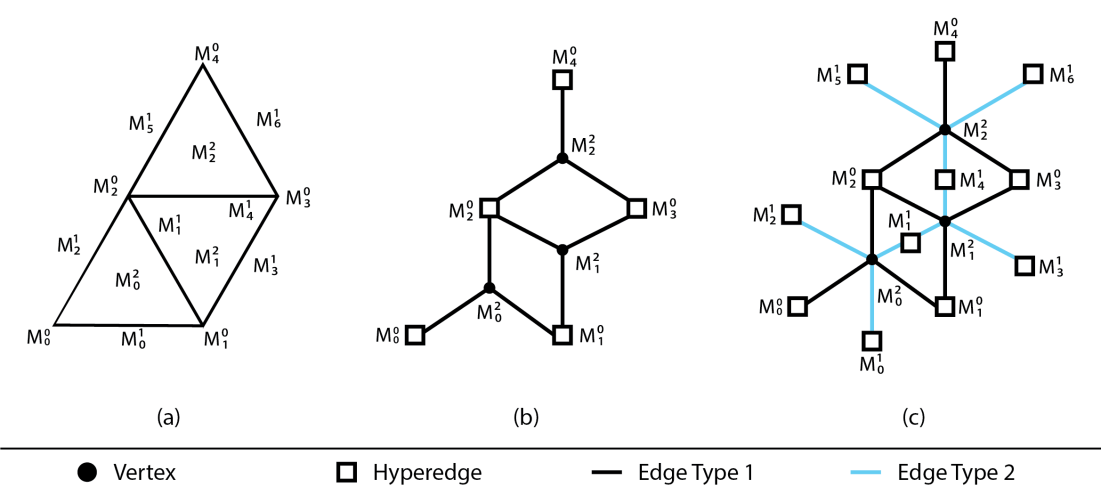
\includegraphics[width=3.5in]{../figures/exampleMesh2Graph.png}
  \caption{(a) a 2D unstructured mesh. (b) N-graph construction with elements$\rightarrow$vertices, vertices$\rightarrow$hyperedges. (c) Same construction, but with an additional edge type for mesh edges.}
  \label{fig:mesh2graph}
\end{figure}

In previous work on this case, we used EnGPar to improve partitions of an
element-partitioned mesh targeting balancing mesh vertices and mesh elements \cite{engparSC17}.
For larger process counts, EnGPar fell short balancing mesh vertices.
We identified that EnGPar was stagnating due to poor choices of destination part
when selecting graph vertices that were on the part boundary of several processes. In order
to make better decisions, we choose the destination part based on the largest surface area
between the source part and the potential destination part. This results in migrating these
vertices to parts that are more connected to the source part instead of parts that may only
share a few edges.

\subsection{Vertex-partitioned meshes}\label{sec:vtxPtn}

To represent the vertex-partitioned mesh in EnGPar, the construction
is essentially the opposite of the element-partitioned mesh. Graph
vertices are defined by mesh vertices and graph hyperedges are defined
by mesh elements. The pins between graph vertices and hyperedges are
created for any mesh vertex that bounds a mesh element.
Alternatively, the hyperedges could be formed from mesh edges or faces.
Defining mesh faces as hyperedges is similar in characteristic to hyperedges
formed from elements; they both have low degree.

During initial attempts at improving the partitions, we found that the edge cut was growing
at a large rate as we improved edge imbalance. This has been attributed to the differences
caused by the vertex-partitioning of the mesh. In an unstructured mesh, vertices have
high degree upward adjacencies while elements have low degree downward
adjacencies: i.e., four vertices bound a tetrahedron, five for a pyramid, six
for a prism, etc. For element-partitioned meshes, the hyperedges
represent the mesh vertices. To maintain a low edge cut, mesh vertices that bound many mesh
elements should not be cut across partitions. Towards this, EnGPar avoids migrating cavities
around these high degree hyperedges by searching for low degree cavities. For vertex-partitioned
meshes, this problem is reversed since mesh vertices are represented as graph vertices
and hyperedges have low degree.
Thus, the problem of edge cut arises from having high degree graph vertices along the partition
boundary which leads to a larger edge cut. To avoid increasing the edge cut, when balancing
elements in the vertex partition we must consider the degree of the vertices that bound the
hyperedges.

To control the edge cut while balancing the graph, we introduce a metric to represent the
potential edge cut change for a cavity. The metric is the ratio of hyperedges that will be cut
after the cavity is migrated to the hyperedges currently cut around the cavity. We use a tunable
parameter in EnGPar that will not migrate a cavity if the metric is above the parameter.
Setting this parameter to 1.0 forces EnGPar to migrate cavities that will not increase the edge
cut locally. This does not guarantee that the edge cut will decrease as the metric does not take
into account other cavities that are migrated in the iteration. Smaller values of this
parameter will limit the increase in edge cut, but also limit EnGPar's ability to improve the
imbalance and either take more iterations to reach the imbalance tolerance or stagnate at a
higher imbalance.

\subsection{Boundary Layer Stacks}

Semi-structured boundary layer element stacks growing from geometric model faces can
be used to reduce discretization errors and reduce mesh element count (i.e., versus
a full unstructured tetrahedral mesh) when there are strong gradients in
fields normal to a geometric model surface.
Localizing a stack of elements, or vertices along the growth curve, can reduce
communications during a PDE solve that uses line relaxation pre-conditioning
methods~\cite{wesseling2001311} for improved convergence, and during mesh
adaptation coarsening procedures~\cite{chitale-aiaa14,Sahn07,loseille20093d}.

Algorithm \ref{alg:collapse} details steps taken to
combine the stacks for a vertex-partitioned mesh. The algorithm loops over each
vertex classified on a geometric
model face to see if it bounds a prism on lines 1-2. From each of these vertices, the
algorithm searches for the mesh edge that does not bound any triangles on lines 5-9. An edge
that only bounds quad faces is guaranteed to be the edge going up the prism elements. If
this edge is found, lines 10-14 find the other vertex that bounds this edge and repeats
looking for a new edge from this vertex. This process is continued until no edge is found
since once a tetrahedron or pyramid element is hit there will be no edges that are
not adjacent to a triangle.
Note, the algorithm is simplified to assume each stack exists on a single
process.
If this were not the case, topological information used to stitch parts
together (i.e., which processes have a copy of a given mesh entity and the
pointer to the entity on the remote process) would be queried and peer-to-peer
communications required to complete the stack traversal.

\begin{algorithm}
  \caption{Boundary Layer Stack Collapse}
  \label{alg:collapse}
  \small
  \begin{algorithmic}[1]
    \ForAll{vertices, $v$, classified on a geometric model face}
    \If{$v$ bounds a prism}
    \State $prev\_edge = NULL$
    \State $next\_edge = NULL$
    \ForAll{edges, $e$, bounded by $v$}
    \If{$e$ bounds no triangles and is not $prev\_edge$}
    \State $next\_edge = e$
    \EndIf
    \EndFor
    \If{$next\_edge$ is not $NULL$}
    \State $edge\_prev = e$
    \State $v = other\_vertex(v,e$)
    \State goto 4:
    \EndIf
    \EndIf
    \EndFor
  \end{algorithmic}
\end{algorithm}

To maintain the correct computational and communication load of the stacks,
we assign weights to the vertices and hyperedges that represent the stack. Each boundary layer
stack vertex accumulates the weight of the mesh vertices in the stack, while the hyperedges
accumulate the weight of the elements that share the same graph vertices. If the
application does not supply per-vertex and per element weights than a unit
weight is assigned.

\section{Results} \label{sec:results}

\subsection{Element-partitioned mesh}

Tests for the finite element case were run with a one billion element
tetrahedral mesh of an airplane's
vertical tail structure. EnGPar was run on the Mira BlueGene/Q system at the Argonne Leadership
Computing Facility \cite{haring2012ibm} on partitions from 128Ki ($128*2^{10}$) up to 512Ki parts.
These partitions were created by using ParMETIS part k-way \cite{karypis1999parallel} globally
up to 8Ki parts. Then METIS is run on each part locally to create the 128Ki to 512Ki partitions.
The initial mesh element imbalance is 2\% and the mesh vertex imbalance ranges from 12\% for
the 128Ki partition up to 53\% at 512Ki parts.

We compare EnGPar to ParMA \cite{SmithParma2015}, a diffusive load balancer that
works directly on an unstructured mesh.
Each tool is run on the partitions with the goal of balancing the mesh vertices down to 5\%
while keeping the mesh
element imbalance below 5\%. Figures \ref{fig:fem_vtximb} shows the mesh vertex imbalance from
ParMETIS and after EnGPar and ParMA are used. Both tools significantly reduce the mesh vertex
imbalance. For the 128Ki and 256Ki cases, both reduce the imbalance to the target 5\%. In
the 512Ki case, EnGPar reduces the mesh vertex imbalance to 6\% while ParMA reduces to the
target.

\begin{figure}[!ht]
  \centering
  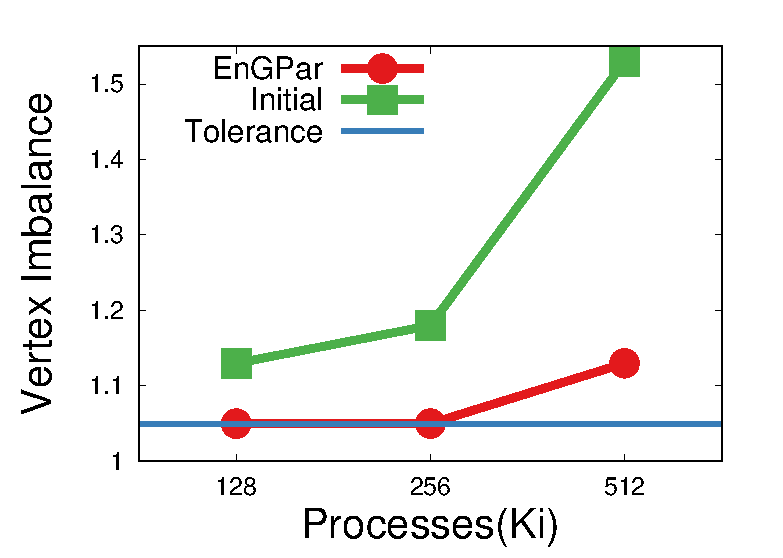
\includegraphics[width=3in]{plots/mira_fem_results/vimb_v_cores}
  \caption{Vertex imbalance for the initial partitioning and the partitions created by
    EnGPar and ParMA. Element imbalance is maintained below the 5\% tolerance for all cases.}
  \label{fig:fem_vtximb}
\end{figure}

Figure \ref{fig:fem_time} shows the runtime for each partition of ParMA and EnGPar. The
timing for EnGPar includes the construction of the N-graph and subsequent repartition of
the mesh after running EnGPar to fairly compare with ParMA which doesn't require any
conversions of the mesh. In all cases EnGPar runs faster. The speedup ranges from
25\% faster at the 256Ki case up to 54\% faster for the 512Ki partition.

\begin{figure}[!ht]
  \centering
  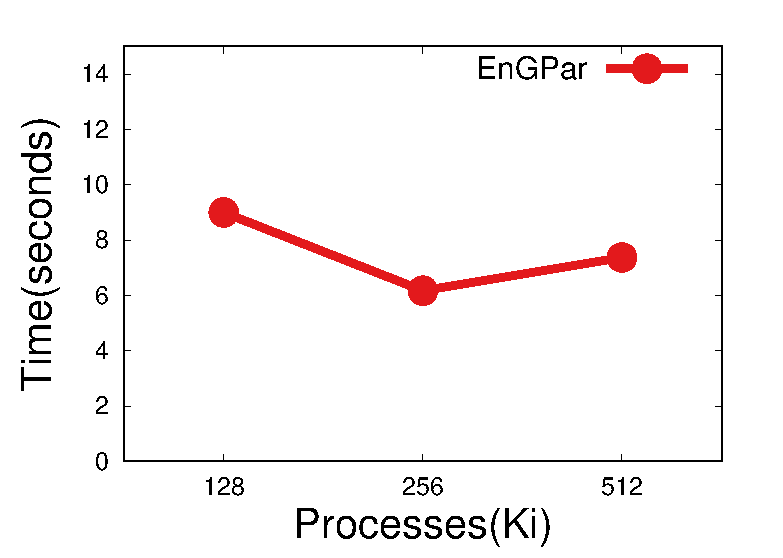
\includegraphics[width=3in]{plots/mira_fem_results/time_v_cores}
  \caption{Time to balance for EnGPar and ParMA}
  \label{fig:fem_time}
\end{figure}

Table~\ref{tbl:avgvtx} shows the average number of vertices in the mesh for each case.
This measurement is related to edge cut in the graph since more average vertices
means more surface area of the part and higher edge cut. ParMA slightly reduces the
vertex counts in every case. EnGPar increases slightly by around 1\% for each case. As was
mentioned for the element-partitioned mesh, the edge cut limit metric was not required to
avoid large increases in edge cut.

\begin{table}[!h]
\centering
\begin{tabular}{||c|c|c|c||}
\hline
&128Ki&256Ki&512Ki \\
\hline
Initial & 2146.404 & 1138.881 & 611.673 \\
ParMA & 2141.965 & 1137.343 & 610.959 \\
EnGPar & 2148.310 &  1143.970 & 619.177 \\
\hline
\end{tabular}
\caption{Average number of mesh vertices per part.}
\label{tbl:avgvtx}
\end{table}

\subsection {Vertex-partitioned mesh}
Experiments for the vertex-partitioned mesh application were done with a 57 million
mixed element mesh (i.e., tetrahedra, prisms, pyramids, and hexahedra) on up to
8192 processes. The mesh is comprised of 32 million tetrahedron,
25 million prisms and 150 thousand pyramids. To show the affect of the edge cut
metric, we ran the same test for each process count using values from 0.5 to 1.2
for the metric limit as well as the metric not being used. Each test runs 30 iterations
of EnGPar's edge balancer while strictly maintaining the vertex imbalance at 5\%.
Figure \ref{fig:metric} shows the edge cut and edge imbalances for each
test; including the initial values of the ParMETIS partitioned mesh. For the
8192 part case, without
the metric used, EnGPar reduces the edge imbalance by 24 percentage points while increasing the cut by
34\%. Turning on the metric with a value of 1.2 results in limiting the increase of the cut to
17\% while reducing the imbalance by 18 percentage points. Results for the metric limit set to 1.0
and 0.8 have similar results following the trend that lower values of the limit result
in lower edge cuts and higher edge imbalance. When the limit is set to 0.5, the edge cut
increases by 1\% while reducing the imbalance by 11 percentage points.

\begin{figure}[!ht]
  \centering
  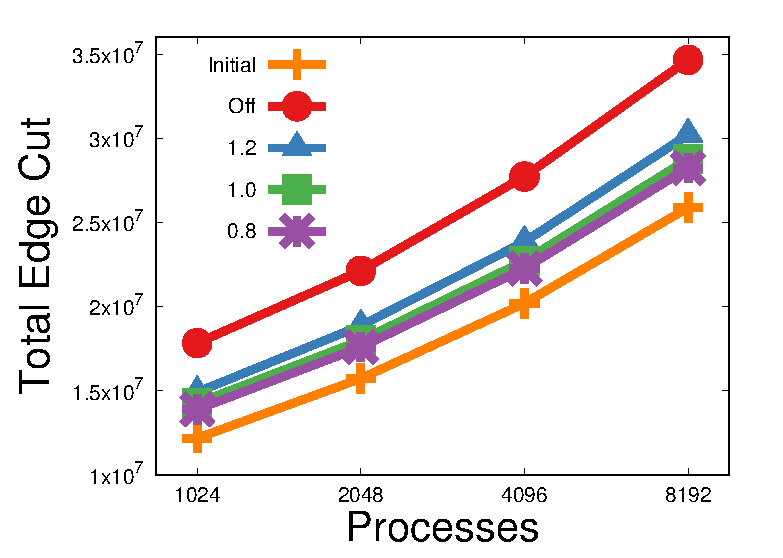
\includegraphics[width=3in]{plots/aepw_edgeCut_collapse_results/ecut_v_cores}
  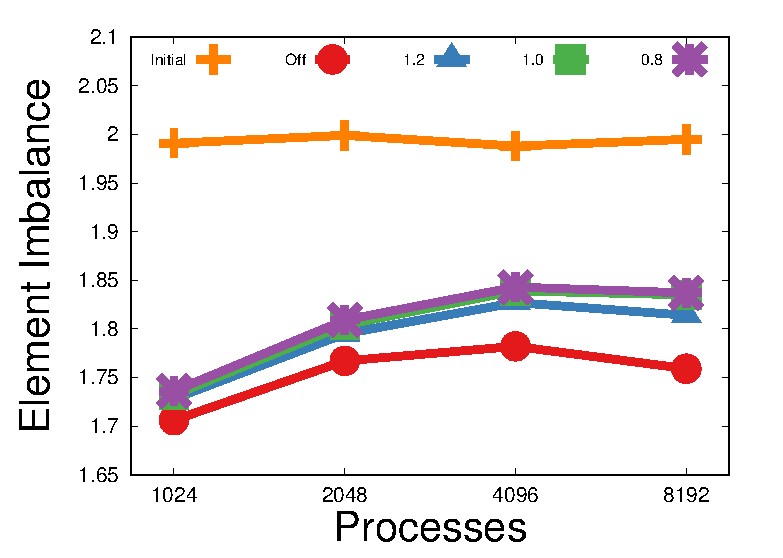
\includegraphics[width=3in]{plots/aepw_edgeCut_collapse_results/eimb_v_cores}
  \caption{Edge cut and imbalance for various values of the metric used to reduce the growth of edge cut. Initial values from ParMETIS and not using the metric are also provided. Vertex imbalance is 5\% for all cases.}
  \label{fig:metric}
\end{figure}

The best edge cut metric parameter is specific to each application. The increase in
edge cut means that there will be more elements on each part as well as
increased communication
between parts. If communication dominates a simulation's scaling then the increase in
edge cut, and the associated increse in communications, may negate, or exceed,
any savings from improved balance. So, the partition from ParMETIS may
be the best choice, or running EnGPar with a low limit for the cut growth metric like in the
0.5 case. However, if the application is very susceptible to imbalance, then a increase in the
edge cut would be worth the larger decreases in imbalance as seen in the 0.8 - 1.2 cases.

For the boundary layer collapse, we use the same 57 million element mixed mesh. The N-graph is
built in serial from the mesh with the collapsed boundary layers and partitioned
out using global ParMETIS for the 1024 to 8192 partitions.
Then, EnGPar is run for 30 iterations to reduce the edge imbalance with the same set of
configurations for the edge cut metric limit. Figure \ref{fig:collapse}
shows the edge cut and edge imbalance after partitioning with
ParMETIS and after EnGPar. Without the metric limit, there is a 41\% point reduction in
element imbalance with a 38\% increase in edge cut. The usage of the metric has a much larger
affect than in the uncollapsed boundary layer case. For a value of 1.2 there is a 35\% point
drop in imbalance with a 15\% increase in edge cut. Similar trends are seen for the 1.0 and 0.8
limit. The 0.5 metric reduces the imbalance by 11 percentage points with a less than 1\% increase in the
edge cut.


\begin{figure}[!ht]
  \centering
  \includegraphics[width=3in]{plots/aepw_edgeCut_collapse_results/ecut_v_cores_collapse}
  \includegraphics[width=3in]{plots/aepw_edgeCut_collapse_results/eimb_v_cores_collapse}
  \caption{Edge cut and imbalance for the graph with collapsed boundary layer stacks. Initial values from ParMETIS are provided. Vertex imbalance is 5\% for all cases.}
  \label{fig:collapse}
\end{figure}

\section{Closing Remarks} \label{sec:closing}


EnGPar was used to improve the partitions of three different application data. A
graph was constructed that compactly represents particles in a fusion application. This
graph was designed such that the partition requirements of particles were always satisfied
regardless of decisions made by EnGPar.
An initial test reduces the particle imbalance by 24 percentage points.
In the future, larger simulations will
be run to further test EnGPar's graph construction and balancing procedures.

Previous results using EnGPar to improve the partitions for an element-based CFD application
were revisited. Improvements were made that further reduced the
imbalance while not sacrificing significant imbalance of the primary vertices,
edge cut, or runtime.

Vertex-partitioned meshes for CFD were considered. The diffusive methods used previously for
element-partitioned meshes were not able to control the edge cut while improving the partitions.
A new metric was introduced that with tuning is able to give a range for trading between edge
cut and imbalance. Additionally, combining boundary layer stacks was explored. The metric for
the edge cut was more effective in decreasing imbalance and limiting the increase in edge cut.

\section{Acknowledgements}

Consultation on CFD methods was provided by members of the NISC SI2-S2I2
Conceptualization of CFDSI: Model, Data, and Analysis Integration for End-to-End
Support of Fluid Dynamics Discovery and Innovation; Award Number 1743185 and 
1743178.

Computational resources and system support were provided by the Rensselaer
Polytechnic Institute Computational Center for Innovations.
An award of computer time was provided by the Innovative and Novel Computational
Impact on Theory and Experiment (INCITE) program and a separate award of
computer time by the Theta Early Science program.
This research used resources of the Argonne Leadership Computing Facility, which
is a DOE Office of Science User Facility supported under Contract
DE-AC02-06CH11357.

\bibliographystyle{IEEEtran}
\bibliography{scorec-refs/scorec-refs}

\appendices

\section{Artifact Description Appendix: 
Dynamic Load Balancing of Plasma and Flow Simulations}

%%%%%%%%%%%%%%%%%%%%%%%%%%%%%%%%%%%%%%%%%%%%%%%%%%%%%%%%%%%%%%%%%%%%%
\subsection{Abstract}

Information is provided to create the vertex partitions of the Aeroelastic
Prediction Workshop mesh that are described in Section~\ref{sec:results} of the ScalA18
workshop paper titled ``Dynamic Load Balancing of Plasma and Flow Simulations''.

%%%%%%%%%%%%%%%%%%%%%%%%%%%%%%%%%%%%%%%%%%%%%%%%%%%%%%%%%%%%%%%%%%%%%
\subsection{Description}

\subsubsection{Check-list (artifact meta information)}

{\small
\begin{itemize}
  \item {\bf Algorithm: } diffusive partition improvement
  \item {\bf Program: } EnGPar
  \item {\bf Compilation: } IBM XL C/C++ Blue Gene/Q, V12.1
  \item {\bf Transformations: } unstructured conformal mesh to hypergraph
  \item {\bf Data set: } DOI: 10.5281/zenodo.1409558 {\color{red} GD please
    create a tarball of the aepw input graphs with an included README and place it on
    a scorec filesystem}
  \item {\bf Hardware: } IBM Blue Gene/Q
  \item {\bf Output: } https://github.com/SCOREC/EnGPar-Docs/tree/master/scala18
    {\color{red} GD please change the url to the git hash of the submitted version}
  \item {\bf Publicly available?: } Yes
\end{itemize}
}

\subsubsection{How software can be obtained}

EnGPar is available on Github.  The following version was used for the
experiments:

{\color{red} GD link to engpar github commit hash}

{\color{red} GD list other versions as needed}

\subsubsection{Hardware dependencies}

The experiments were performed on the IBM Blue Gene/Q at Argonne National
Laboratories and Rensselaer Polytechnic Institute's Center for Computational
Innovations.

\subsubsection{Software dependencies}

EnGPar calls ParMETIS XYZ to perform initial partitioning.
{\color{red} GD WHAT VERSION OF PARMETIS? 4.0.3 ?}

{\color{red} OTHER DEPS?}

\subsubsection{Datasets}

The Zenodo datasets containing the input graphs of the Aeroelastic Prediction
Workshop mesh are available at 10.5281/zenodo.1409558 .

%%%%%%%%%%%%%%%%%%%%%%%%%%%%%%%%%%%%%%%%%%%%%%%%%%%%%%%%%%%%%%%%%%%%%
\subsection{Installation}

{\color{red} GD please provide environment files, build scripts, and commands
used to build engpar on CCI BGQ}

%%%%%%%%%%%%%%%%%%%%%%%%%%%%%%%%%%%%%%%%%%%%%%%%%%%%%%%%%%%%%%%%%%%%%
\subsection{Experiment workflow}

{\color{red} GD please provide job submission scripts and commands
used to run engpar on CCI BGQ}

%%%%%%%%%%%%%%%%%%%%%%%%%%%%%%%%%%%%%%%%%%%%%%%%%%%%%%%%%%%%%%%%%%%%%
\subsection{Evaluation and expected result}

Expected results are located in the 
https://github.com/SCOREC/EnGPar-Docs/tree/master/scala18
repo.
{\color{red} LINK TO SUBMITTED VERSION}

Plots of vertex and edge imbalances and edge cut are produced by
running the bash script \texttt{parseAndPlot.sh} in the
\texttt{scala18/plots/aepw_edgeCut_collapse_results} directory.
GNUPlot is required for plotting.

\section{Artifact Evaluation Appendix: Dynamic Load Balancing of Plasma and Flow Simulations}

%%%%%%%%%%%%%%%%%%%%%%%%%%%%%%%%%%%%%%%%%%%%%%%%%%%%%%%%%%%%%%%%%%%%%
\subsection{Abstract}

Results were verified through multiple runs using the same partition of nodes.

{\color{red} GD can you confirm this for the aepw results?}

%%%%%%%%%%%%%%%%%%%%%%%%%%%%%%%%%%%%%%%%%%%%%%%%%%%%%%%%%%%%%%%%%%%%%

\subsection{Results Analysis Discussion}

{\em Description of results, their correctness and any concerns about them. If your paper is only about performance, describe how you assure the quality of performance measurements and that you have preserved correct computational results.}

EnGPar's performance is evaluated using timers around high-level routines that
take several seconds to execute and graph based quality metrics.
Our timers call \texttt{MPI\_Wtime} on the IBM Blue Gene/Q which are implemented
in IBM's MPI with high precision system clock based timers.
Any timing runs are repeated multiple times and {\color{red} GD what do we do then? average?
max?}.
Graph partition qualtiy metrics are verified against the same metrics computed
directly on mesh entities by ParMA.

The source code for EnGPar's timers and metrics are HERE and HERE, respectively.
{\color{red} GD please add links}.

%%%%%%%%%%%%%%%%%%%%%%%%%%%%%%%%%%%%%%%%%%%%%%%%%%%%%%%%%%%%%%%%%%%%%
\subsection{Summary}

{\em Final summary demonstrating the trustworthiness of your results.}

We provide full source code with the specific Git SHA1 and inputs to reproduce
our results.
Nightly builds and tests are run to prevent regressions.

{\color{red} GD any other ideas?}


\end{document}
